\documentclass[addpoints,11pt]{exam}

\usepackage{alltt}
\usepackage[margin=1in]{geometry}   % set up margins
\usepackage[T1]{fontenc}
\usepackage[usenames,dvipsnames]{xcolor}
\usepackage{enumerate}              % fancy enumerate
\usepackage{amsmath}                % used for \eqref{} in this document
\usepackage{amsthm}
\theoremstyle{definition}
\newtheorem{exmp}{Example}[section]
\usepackage{verbatim}               % useful for \begin{comment} and \end{comment}
\usepackage{eurosym}                % used for euro symbol
\usepackage{caption} 
\usepackage{graphicx}
\graphicspath{{Figures/}}
\usepackage{subcaption}
\usepackage{color}
\usepackage{float}
\usepackage{amssymb}
\usepackage{sgamevar}
\usepackage{sgame}
\usepackage[colorlinks=true]{hyperref}
\hypersetup{colorlinks=true, citecolor=ForestGreen, linkcolor=BlueViolet, urlcolor=Magenta}



%Solutions or nah (blank next two lines out for no solutions, unblank #3)
%\printanswers
%\newcommand{\dd}[1]{\par {\textbf{\textcolor{red}{#1}}}}
\newcommand{\dd}[1]{}  


\setlength\parindent{0pt}
\unframedsolutions
\SolutionEmphasis{\color{red}}
\CorrectChoiceEmphasis{\color{red}}
\renewcommand{\choicelabel}{(\alph{choice})}
\newcommand{\blank}[0]{\underline{\hspace{3cm}}}
\pointformat{\bfseries[\thepoints]}
\pointpoints{pt}{pts}
\pointsinrightmargin


\begin{document}
	
	
	\title{\textbf{Homework 6} \\ \dd{Solutions\\} \vspace{2 mm} {\large ECON 101}}
	\author{Summer I 2016}
	\date{}
	\maketitle
	
\makebox[\textwidth]{Name:\enspace\hrulefill}
\\

\makebox[\textwidth]{ONYEN:\enspace\hrulefill}
\\

\makebox[\textwidth]{PID:\enspace\hrulefill}
\\

\begin{center}
	\fbox{\fbox{\parbox{5.5in}{\centering
	This (optional) homework is due on \textbf{June 14} by \textbf{11AM}. Show work for all questions that require it (including multiple choice questions), attaching extra sheets as necessary. Multiple choice answers should be bubbled in on a scantron. For the short answer section, write legibly and make sure to box final answers. The total number of points available on this assignment is \textbf{40}.}}}
\end{center}
	
	\subsection*{Multiple Choice [2 pts each]}

\begin{questions}


\question When the economy goes into a recession, real GDP \blank and unemployment \\ \blank.

\begin{choices}
	\choice rises; rises
	\choice rises; falls
	\CorrectChoice falls; rises
	\choice falls; falls
\end{choices}



\question A change in the expected price level shifts 

\begin{choices}
	\choice the AD curve.
	\CorrectChoice the short-run AS curve, but not the long-run AS curve.
	\choice the long-run AS curve, but not the short-run AS curve. 
	\choice both the short-run and the long-run AS curve.
\end{choices}

\begin{solution}
	The SRAS curve is determined by $\pi^e$, while the LRAS curve is determined by the natural growth rate.
\end{solution}

\question An increase in the AD for goods and services has a larger impact on output  \blank  and a larger impact on the price level \blank.

\begin{choices}
	\CorrectChoice in the short run; in the long run
	\choice in the long run; in the short run
	\choice in the short run; also in the short run
	\choice in the long run; also in the long run
\end{choices}

\begin{solution}
	An increase in AD will cause output and inflation to rise in the short run. In the long run, inflation will increase further, but output will return to its natural growth rate.
\end{solution}

\newpage

\question Sticky wages and prices 

\begin{choices}
	\choice reduce the impact of negative shocks.
	\CorrectChoice increase the impact of positive shocks.
	\choice have no effect on the impact of negative shocks. 
	\choice offset the impacts of positive shocks.
\end{choices}

\begin{solution}
	Sticky wages and prices increase the impact of both positive and negative shocks. A stickier SRAS curve will have a larger impact on SR real growth in either case.
\end{solution}

\question Imagine that a government starts out with a budget surplus. If in the next period the government temporarily runs a budget deficit, what would you expect to happen to aggregate demand?

\begin{choices}
	\CorrectChoice AD would increase.
	\choice AD would lie at the natural growth of output.
	\choice AD would be unchanged.
	\choice AD would decrease. 
\end{choices}

\begin{solution}
	A budget deficit would come about because (i) G increased, (ii) taxes decreased, or both. Either way, spending increases and so AD increases.
\end{solution}


\question If the central bank wants to expand aggregate demand, it can \blank the money supply, which would \blank the interest rate.

\begin{choices}
	\choice increase; increase
	\CorrectChoice increase; decrease
	\choice decrease; increase
	\choice decrease; decrease
\end{choices}

\begin{solution}
	The Fed increases the money supply through open market purchases (buying bonds). Increased demand for bonds raises their price, which in turn decreases the interest rate on those bonds.
\end{solution}

\question Which of the following is an example of an automatic stabilizer? When the economy goes into a recession,

\begin{choices}
	\CorrectChoice more people become eligible for unemployment insurance benefits.
	\choice stock prices decline, particularly for firms in cyclical industries.
	\choice Congress begins hearings about a possible stimulus package.
	\choice the Fed changes its target for the federal funds rate.
\end{choices}



\question When consumers are very reluctant to spend in a recessionary environment, the government's most effective strategy is to 

\begin{choices}
	\CorrectChoice increase spending through bond financing.
	\choice decrease income taxes.
	\choice decrease corporate taxes.
	\choice do nothing - the economy will self-correct in the short run.
\end{choices}

\begin{solution}
	Government spending is most effective if consumer's are reluctant to spend. Decreasing taxes may not spur spending if most individuals choose to save their extra income.
\end{solution}

\newpage

\question Consider Figure \ref{fig1}.


\begin{figure}[H]
	\centering
	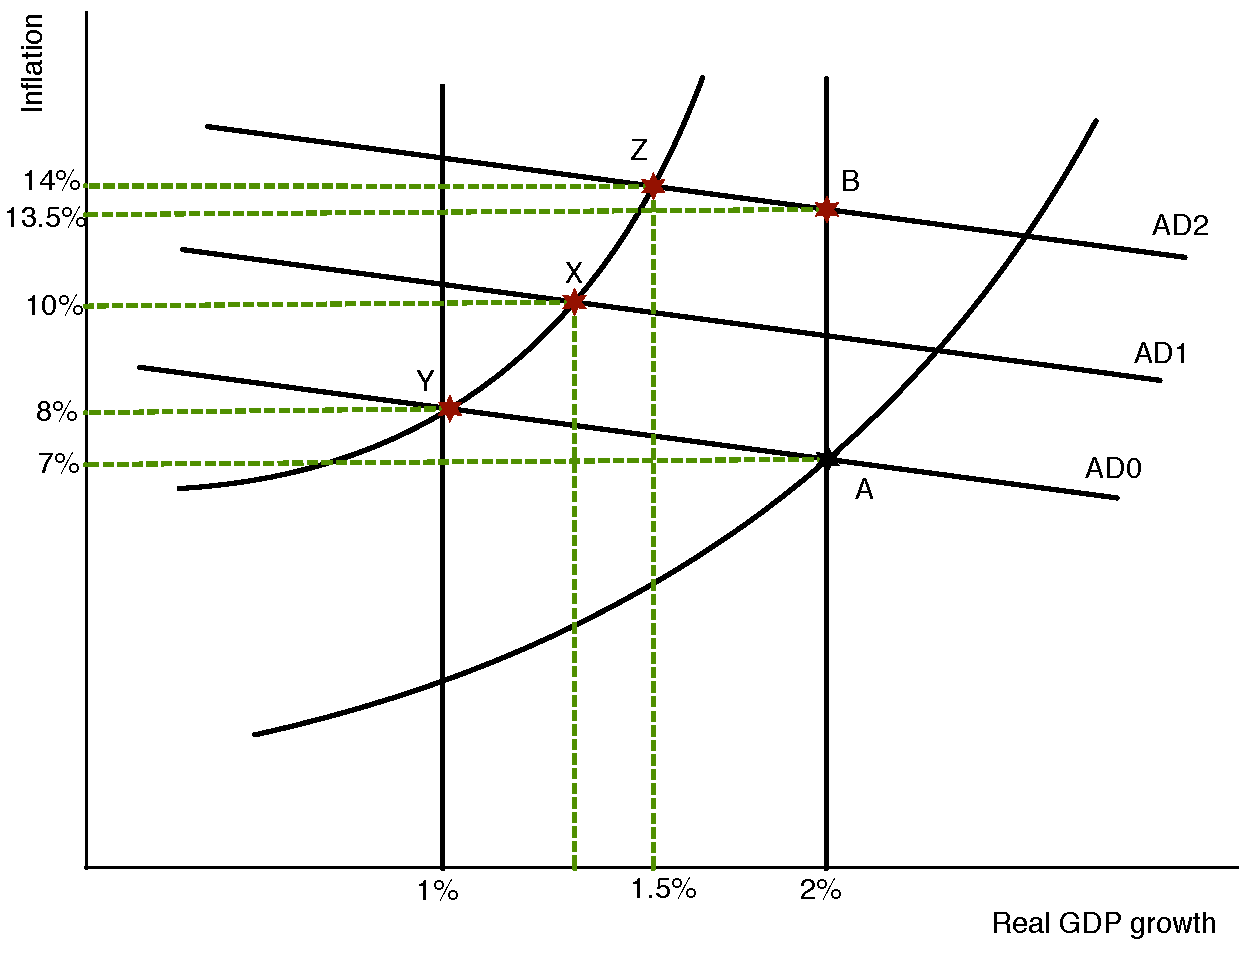
\includegraphics[scale=.45]{ec2_plot1.pdf}
	\caption{Real Shock}
	\label{fig1}
\end{figure}

If after a real shock the economy is operating at point $Y$, then, in the absence of crowding out, fiscal policy that shifted $AD0$ to $AD2$ would move the economy to point

\begin{choices}
	\choice $A$
	\choice $B$
	\CorrectChoice $Z$
	\choice $X$
\end{choices}

\begin{solution}
	Real shock moved LRAS curve from $g=2\%$ to $g=1\%$. Long-run Eq at $AD0$ is $Y$. If AD shifts to $AD2$, economy would be where $AD2$ and the new SRAS curve intersect at point $Z$.
\end{solution}

\item If the government wants to contract aggregate demand, it can \blank government purchases or \blank taxes.

\begin{choices}
	\choice increase; increase
	\choice increase; decrease
	\CorrectChoice decrease; increase
	\choice decrease; decrease 
\end{choices}

\begin{solution}
	The government can contract AD by either decreasing their own spending or raising taxes.
\end{solution}

\end{questions}

\newpage

\section*{Short Answer}

\begin{questions}


\question Use Figure \ref{fig2} to answer the questions that follow. Assume that firms are changing the price of final goods at the same rate as inflation.


\begin{figure}[h!]
	\centering
	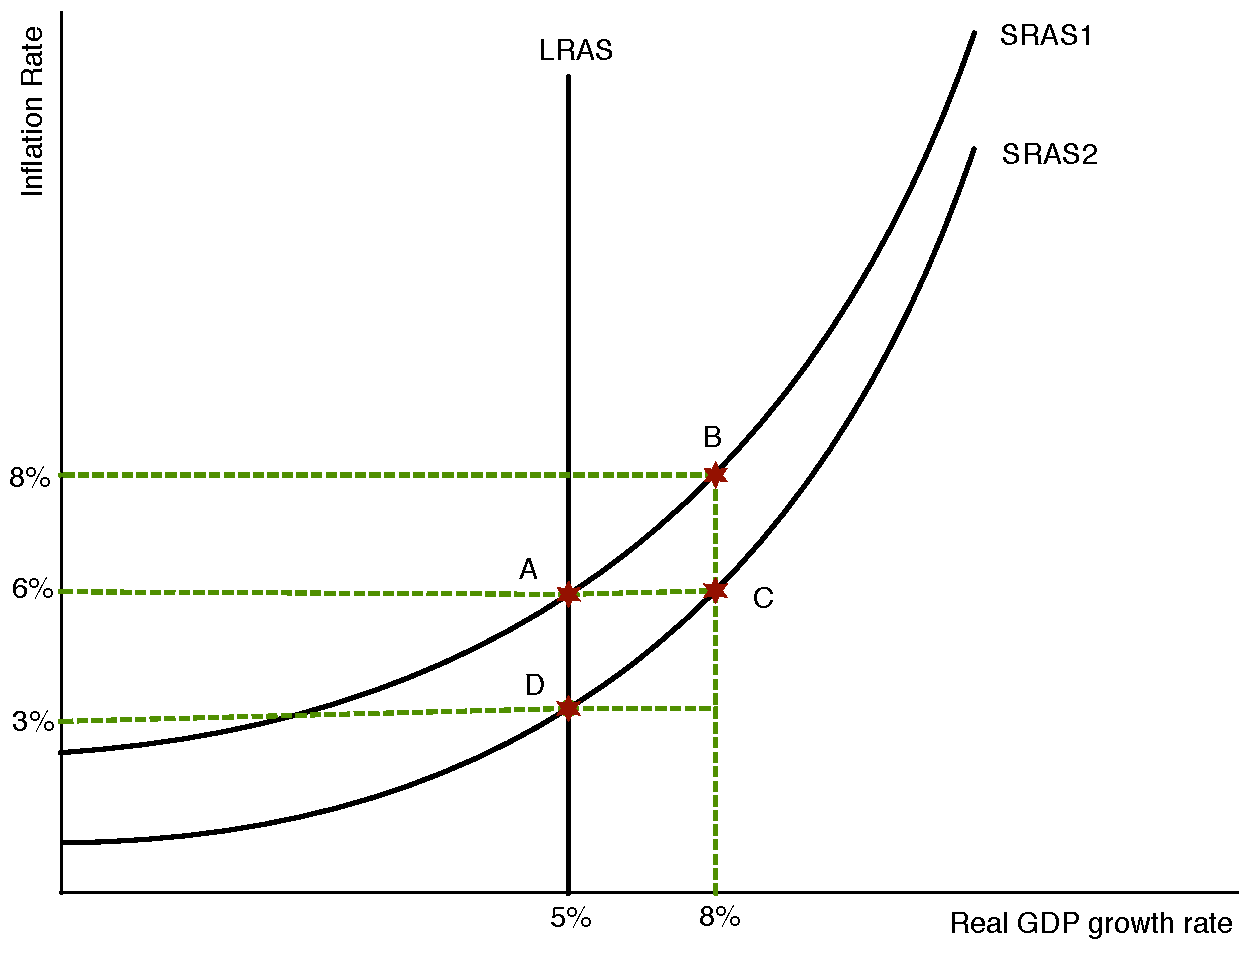
\includegraphics[scale=.45]{hw8_plot1.pdf}
	\caption{SRAS}
	\label{fig2}
\end{figure}

\begin{parts}
	\part[2] If nominal wages are growing at 3\% annually, then at point D how fast are real wages growing? 
	\begin{solution}
		At point D, $\pi = 3\%$. $\%\Delta \text{real wages} = \%\Delta\text{nom. wages} - \pi = 3\% - 3\% = 0\%$.
	\end{solution}
	\part[2] If nominal wages are growing at 3\% annually, then at point C how fast are real wages growing? 
	\begin{solution}
		At point C, $\pi = 6\%$. $\%\Delta \text{real wages} = 3\% - 6\% = -3\%$.
	\end{solution}
	
	\part[2] If nominal wages are growing at a constant rate, what happens to firm profits between points D and C? How will the change in profits affect the growth rate of output?
	
	\begin{solution}
		Between points D and C, firm profits are increasing because expected inflation is less than actual inflation. Prices are rising faster than wages, and so firm profits grow. The growth rate of output will increase to 8\%.
	\end{solution}
	\part[2] Assume we are at point C, and workers are at the point where they can renegotiate wages. In order to maintain the same standard of living that they had at point D, what wage growth rate will they negotiate? 
	\begin{solution}
		At C, $\pi = 6\%$ and so workers will demand nominal wage growth of 6\% in order to return to real wage growth of $0\%$.
	\end{solution}
	\part[2] Will the economy remain at point C? Why or why not? If the point does change, what will the new point be? 
	\begin{solution}
		No. As $\pi^e$ increases, the SRAS curve will shift up until $\pi^e = \pi$ at point A.
	\end{solution}
\end{parts}

	\question Suppose that an economy has a natural growth rate of 2\%. Moreover, the central bank in the country has perfect control over the money supply and increases it by 4\% every year. Assume spending is such that the velocity of money is constant over time and that the economy is currently at its long-run equilibrium.
	
	\begin{parts}
		
		\part[2] Draw a clearly labeled dynamic AS-AD diagram that shows the long-run equilibrium point, as well as the economy's current growth rate of real GDP, inflation, and expected inflation. Label this point $E_0$. Be sure to include both the short-run and long-run aggregate supply curves. 
		
		\begin{solution}
			Long-run equilibrium is where AD, LRAS, and SRAS meet. LRAS is at real GDP growth of 2\%. Spending growth = $\vec{M} + \vec{v} = 4\%$ since $\vec{v} = 0\%$ and money growth is 4\%. By the Quantity Theory of Money, $\vec{M} + \vec{v} = \vec{Y} + \pi$. Since $\vec{Y} = 2\%$, it must be that inflation in the long run is 2\%. Finally, $\pi^e = \pi = 2\%$ at the long run equilibrium.
		\begin{figure}[H]
			\centering
			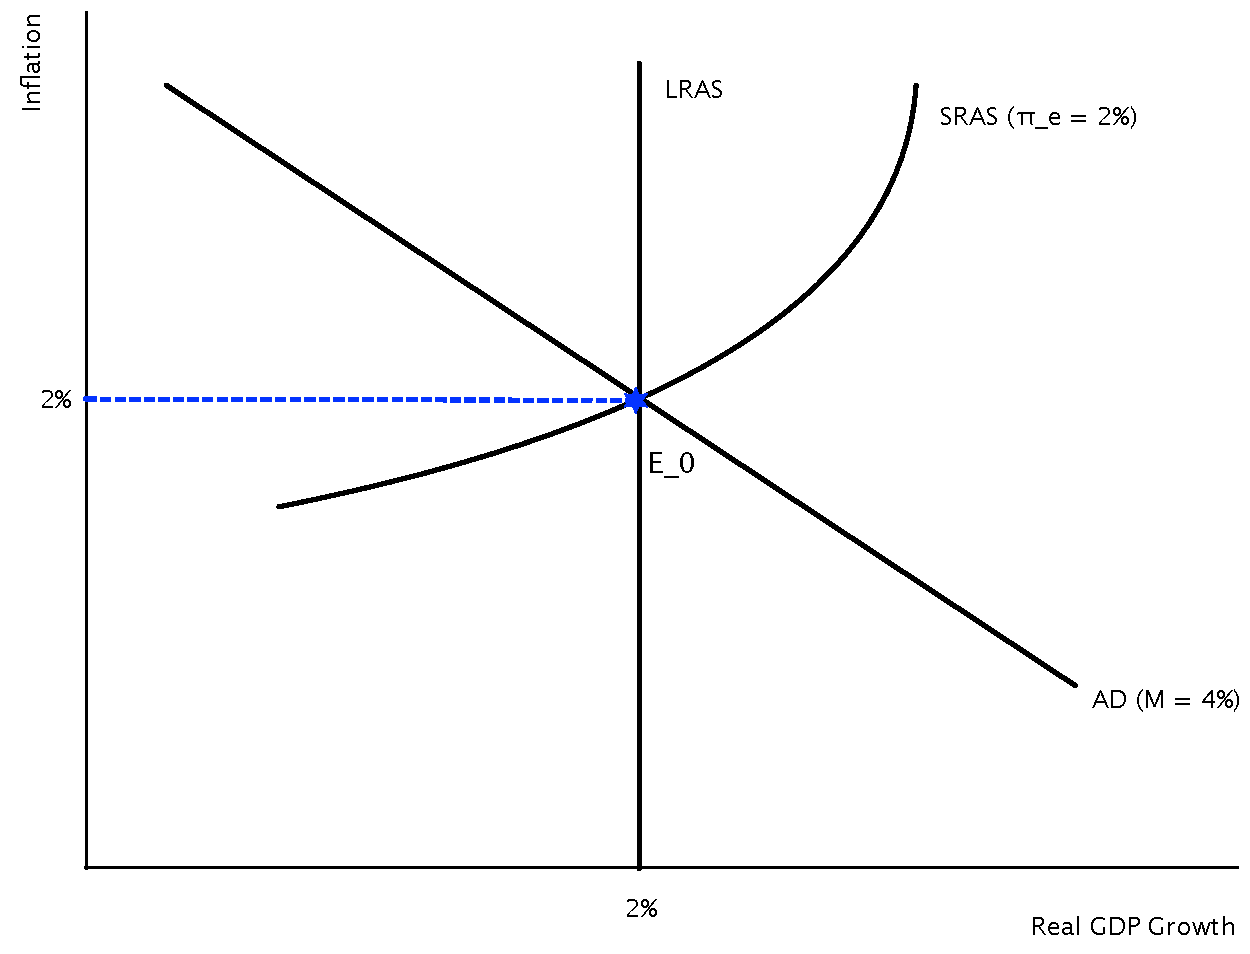
\includegraphics[scale=.45]{hw6_plot1.pdf}
			\caption{AS-AD Model}
		\end{figure}
		\end{solution}
		
		\part[2] Now, suppose that the stock market declines sharply, reducing consumers' wealth. As a result, consumers spend at a rate that is 4\% lower than before. Assume this change is permanent. Does this affect aggregate demand, short-run aggregate supply, or long-run aggregate supply? Explain why. 
		
		\begin{solution}
			This would affect aggregate demand because it would impact consumption spending. Now, $\vec{v} = -4\%$.
		\end{solution}
		
	
		\part[2] Show this change graphically. Assume that neither the central bank nor the federal government enact any policies to counteract this change. Label the short-run equilibrium point $A$ and the long-run equilibrium point $E_1$. What is the inflation rate in the short run if this change in consumer spending caused real GDP growth to decrease to $-1\%$? What will be the long-run real GDP growth rate and inflation rate? 
		
		\begin{solution}
			This decrease in AD is shown in Figure \ref{fig4}. AD shifts left to the AD curve where $\vec{M} + \vec{v} = 4\% + (-4\%) = 0\%$. The short-run point is where the new AD curve and the old SRAS curve meet at point A. If real GDP growth is $-1\%$ at this point, then short-run inflation must be 1\% since spending growth is 0\%. The long-run point $E_1$ is given by where the new AD curve meets the LRAS curve. Long-run growth is the natural rate of 2\%. Since spending growth is 0\%, long-run inflation must be $-2\%$.

		
		
		\begin{figure}[H]
			\centering
			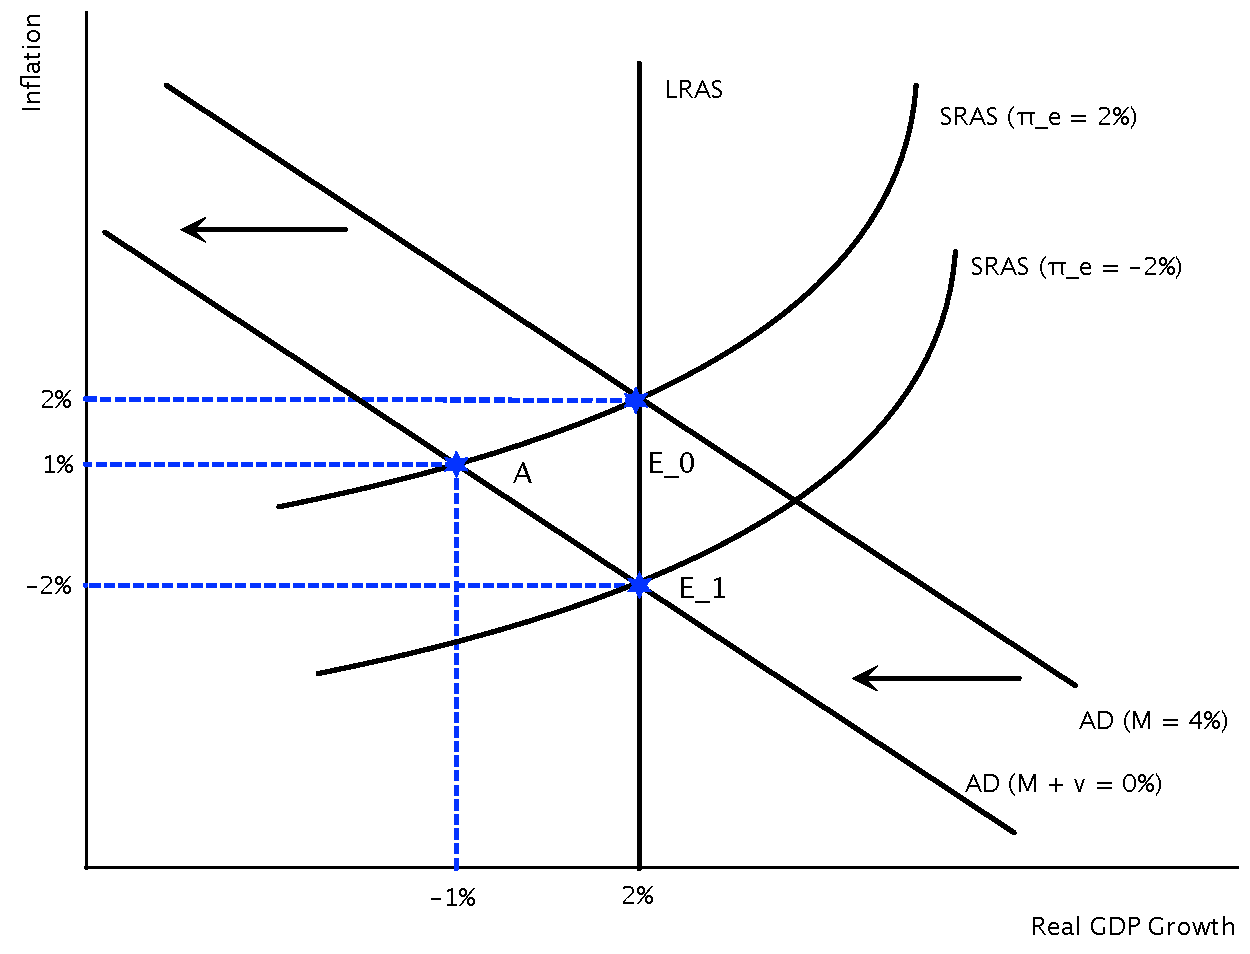
\includegraphics[scale=.45]{hw6_plot2.pdf}
			\caption{Decrease in AD}
			\label{fig4}
		\end{figure}
	
				\end{solution}
		\part[2] Explain why the short-run growth rate of output is different from the long-run growth rate of output. What causes the economy to move from point $A$ to point $E_1$? 
		
		\begin{solution}
			At point A (the short run), actual inflation is less than expected inflation. Thus, firm wages are rising faster than prices and thus firm profits are falling. Due to this, firms will decrease production and in turn real GDP growth will fall. Movement to the long-run point will occur when expected inflation changes to the new long-run inflation rate and the SRAS curve shifts to the right.
		\end{solution}

		\part[2] Suppose the central bank decides to intervene while the economy is at point $A$ in order to get the economy back to point $E_0$. Regardless of the policy pursued, show how this policy would be reflected graphically. Specify what the growth rate of the money supply must be in order for this policy to achieve its goal. 
		
		\begin{solution}
			In order to shift the economy back to point $E_0$, the Fed has to increase aggregate demand. To do so, it must return spending growth to 4\%. If $\vec{v} = -4\%$, then the new growth rate of money the Fed must impose is 8\% since $8\% + (-4\%) = 4\%$.
		
		
		\begin{figure}[H]
			\centering
			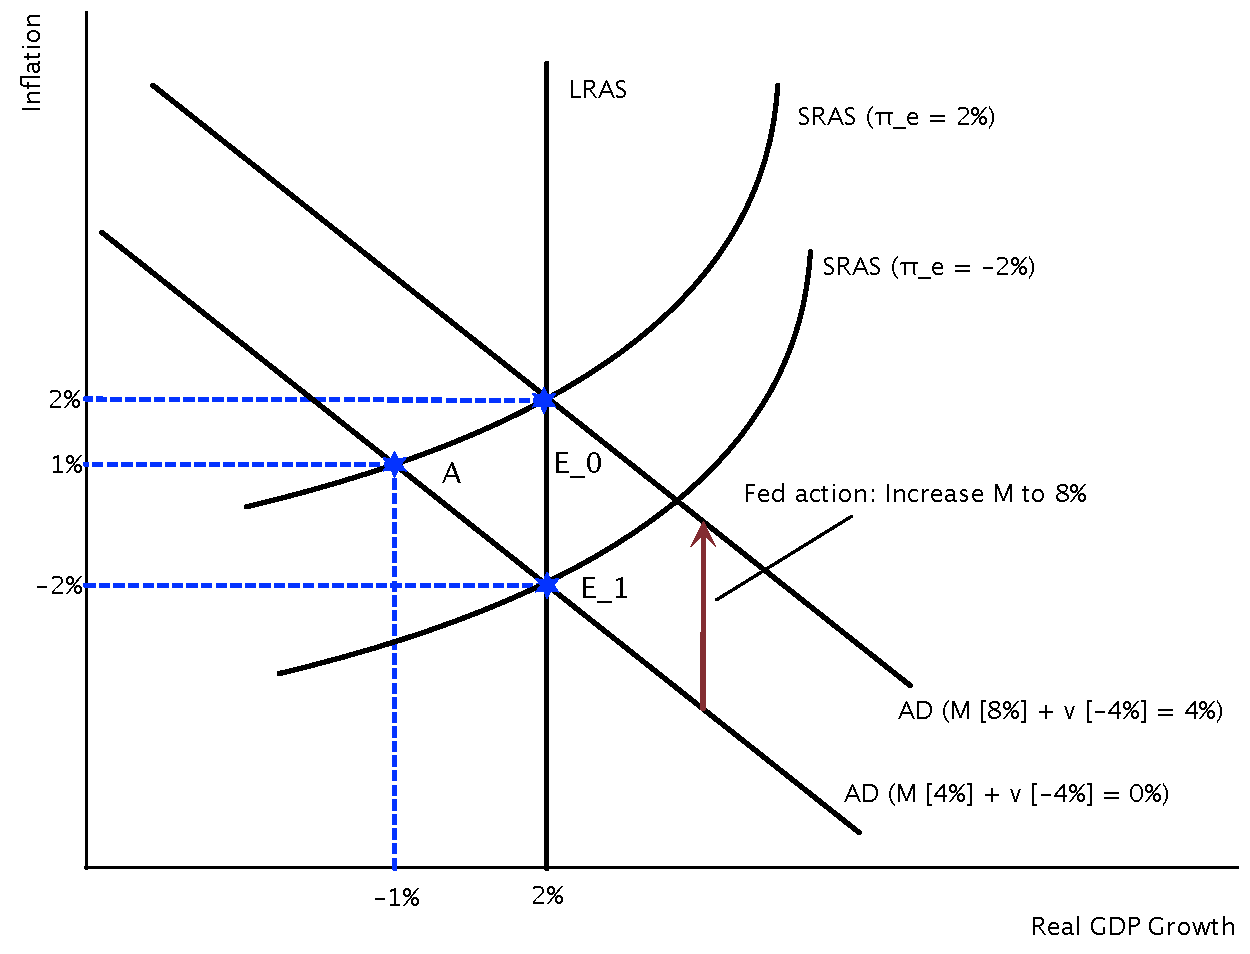
\includegraphics[scale=.45]{hw6_plot3.pdf}
			\caption{Fed Action}
		\end{figure}
		
		\end{solution}
		
	\end{parts}

	\question What topics or questions gave you the most trouble on this homework assignment or the class material it encompassed? 

\end{questions}


\end{document}